When carrying out experimental tests of a model ship at SSPA, a free roll decay test is normally performed to check the properties of the tested ship model.
The roll decay test are conducted by forcing the model to an initial roll angle and then release it to oscillate freely in six degrees of freedom. The tests are conducted either  at zero speed or at speed with a fixed rudder angle. The scaled ship models are between 3 and 6 meters of length. The measurement accuracy of these model tests is very good. When time series from 20 sets of repeated tests were investigated the average $R^2$ was 0.995. The tests were originally conducted in commercial projects for new buildings of merchant ships. In this study, data collected between 2005 and 2018 has been used to construct the roll decay test database, which is applied to build a roll damping database. The main parameters and ship types of ships in the roll decay test database are summarized in Appendix \ref{app:ships}. 

The parameter identification technique was used to estimate the roll damping coefficients from the roll decay tests. It was investigated whether the linear model Eq.( \ref{eq:roll_decay_equation_himeno_linear}), quadratic model Eq.(equation \ref{eq:roll_decay_equation_himeno_quadratic_b}) or cubic model Eq.(\ref{eq:roll_decay_equation_cubic}) was best suited to describe the roll damping of all the test to formulate the roll damping database. After identified the parameters, the corresponding roll motions are simulated by the three mentioned models. The accuracy of the three models was evaluated with the $R^2$ score coefficient, based on model test and simulation time series of roll motions.
The average $R^2$ is 0.995 for the cubic model, 0.993 for the quadratic and 0.986 for the linear model. In addition, Fig. \ref{fig:roll_decay_model_compare} shows a comparison between the models for one of the roll decay test. It can be seen that the linear model can not give a good representation for the whole range of roll motions, and the difference becomes obvious after the time of 30s. Since the quadratic model has almost the same accuracy as the cubic model it was selected to estimate the roll damping from all the roll decay tests in the database. All the extracted roll damping coefficients together with various ship related information will be formulated as the roll damping database for the following analysis.



\begin{figure}[H]
    \centering
    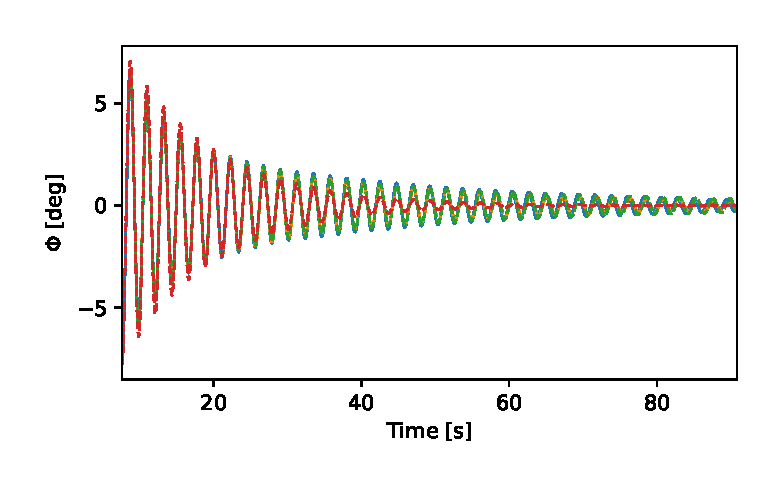
\includegraphics[width=12cm, height = 6cm ]{figures/roll_decay_model_compare.eps}
        \vspace{-0.5cm}
    \caption{Roll decay test comparison of linear (bottom), quadratic (middle) and cubic model (upper).}
    \label{fig:roll_decay_model_compare}
\end{figure}